
The likelihood of female students selecting specific university majors varies significantly based on the gender composition within their classrooms, as evidenced by the series of figures presented.

\vspace{5mm}
\textit{Female Students Choosing  not to Pursue Further Studies}
\vspace{5mm}

Furthermore, the odds ratio for female students choosing not to pursue further studies also varies with changes in the male composition fraction in the classroom. The overall sample odd ratio for female students not pursuing any further studies is 0.101. However, when the proportion of male students is less than 14\%, the odds ratio decreases to around -0.2. This indicates that the likelihood of female students not continuing their studies increases as the proportion of male students in the classroom increases. This relationship is visually depicted in Figure \ref{fig:no_studies}, illustrating how the likelihood of a female student choosing not to pursue further studies shifts in response to variations in the gender composition of the classroom. 



\begin{figure}[H]
\centering
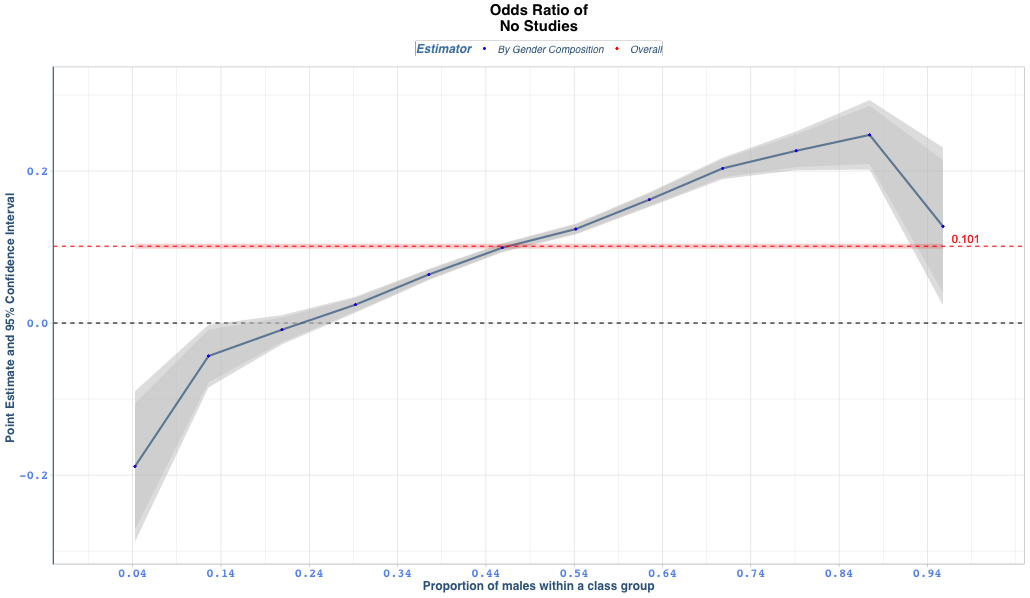
\includegraphics[width=0.8\textwidth]{Graph/Results/fe_panel_student_gender_composition_wome_in_NO_STUDIES_bce.png}
\caption{Likelihood of a female student choosing not to pursue further studies}
\label{fig:no_studies}
\end{figure}
% \subsubsection{Empirical Strategy} \label{empirical_design}

Additionally, when a female school transitions to a coeducational school, the proportion of women who cease studying in the two years following the change tends to increase. This trend is demonstrated in Figure \ref{fig:staggered_females_no_studies}, highlighting the impact of school gender composition changes on female students' study decisions."

\begin{figure}[H]
    \centering
        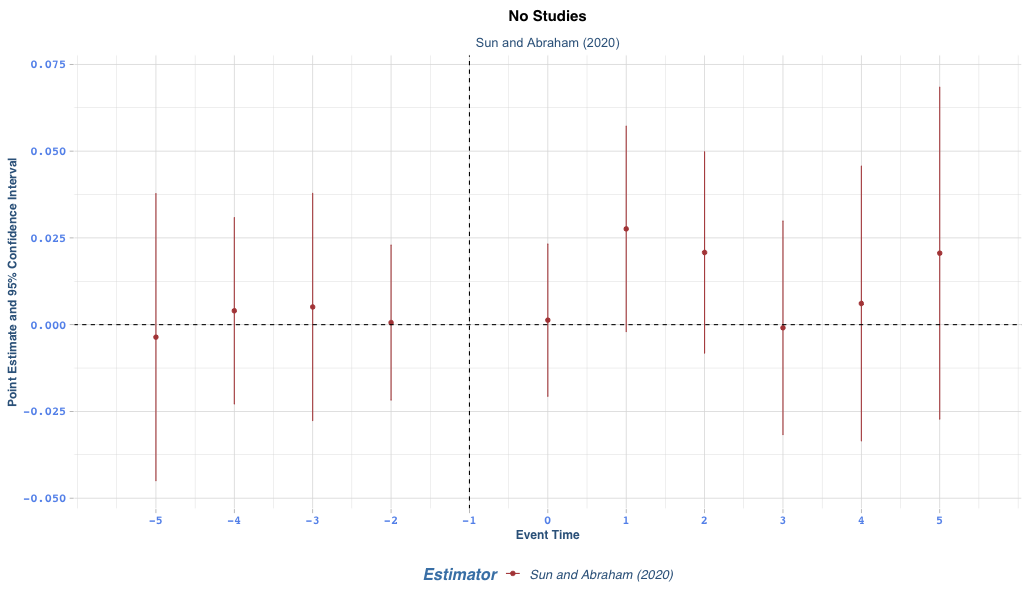
\includegraphics[width=0.8\textwidth]{Graph/Results/stagered_ex_females_NO_STUDIES.png}
        \caption{Proportion of Female Students Not Pursuing Further Studies in Schools Transitioning from Female to Coeducational}
    \label{fig:staggered_females_no_studies}
\end{figure}

\vspace{5mm}
\textit{Female Students Choosing STEM Studies}
\vspace{5mm}


We found that the odds ratio of female students choosing a STEM career reaches 0.92, indicating a significant difference compared to male students in similar classroom compositions. The relationship between classroom gender composition and female students' propensity to pursue STEM studies is depicted in Figure \ref{fig:STEM_studies}, which illustrates how the likelihood of a female student choosing a STEM-related career varies across different proportions of male students in the classroom.

\begin{figure}[H]
\centering
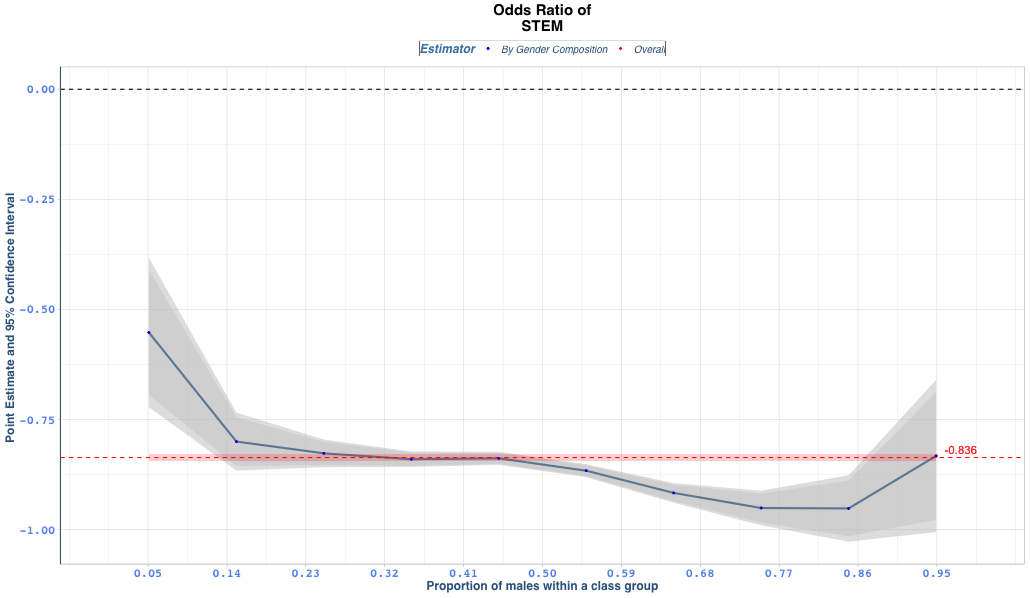
\includegraphics[width=0.8\textwidth]{Graph/Results/fe_panel_student_gender_composition_wome_in_STEM_bce.png}
\caption{Likelihood of a female student choosing a STEM-related career}
\label{fig:STEM_studies}
\end{figure}

When the proportion of male students in the classroom increases, the likelihood of female students opting for STEM-related careers decreases. This finding aligns with existing theories that suggest a correlation between classroom composition, gender dynamics, and career aspirations \citep{Gneezy2003, Thomas2014}. Specifically, in mixed-gender environments, the disparity in competitiveness between men and women tends to widen, with higher levels of competitiveness often associated with a greater inclination towards STEM careers \citep{Thomas2014}.





\begin{figure}[H]
    \centering
        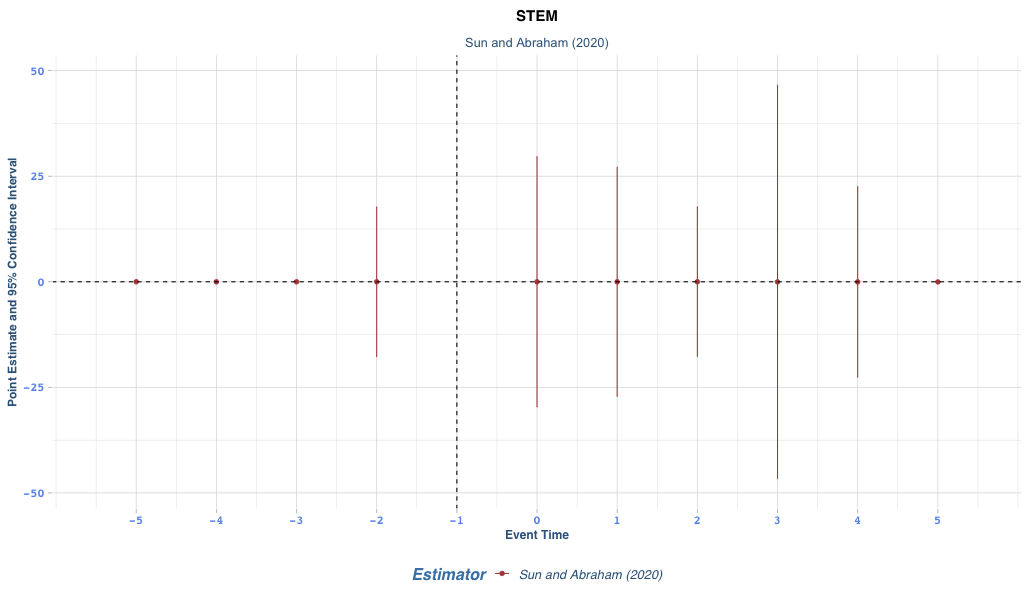
\includegraphics[width=\textwidth]{Graph/Results/stagered_ex_females_STEM.png}
        \caption{Proportion of Female Students Choosing STEM Majors in Schools Transitioning from Female to Coeducational}
    \label{fig:staggered_females_STEM}
\end{figure}

 
 

 